\section{Model}
In this section we describe the model that is used to find the recommended speed.
See Figure~\ref{fig:Introduction:network} for references.

\subsection{Vehicles}
A vehicle, $\veh$, is an entity that moves along a route.
Each vehicle has an identifier, $\vehid$ a maximum speed, $\vehvel$, a constant acceleration, $\vehacc$ and deceleration, $\vehdec$ and a current position, \vehpos. The position is either an edge or a connection (See below) and is updated as the vehicle moves.
For simplicity we do not consider different drivering behaviours, but operate with two types of vehicles: cars and trucks. See Table \ref{table.vehicleTypes} for their specifications.
\begin{table}
\centering
\begin{tabular}{|l|l|l|}\hline
		& Car 	& Truck \\\hline
Max speed 	& 	& \\\hline
Acceleration 	&	& \\\hline
Deceleration 	&	& \\\hline
\end{tabular}
\caption{Types of vehicles}\label{table.vehicleTypes}
\end{table}

\subsection{Connections}
An intersection is made up of several \textit{connections} that connect road segments one can drive to and from.
For example each possible legal pass through the intersection in Figure~\ref{fig:Introduction:network} is a connection as shown in the connection table in Table~\ref{tab:Introduction:connectionTable}. 
A connection, $\con$ is hence unidirectional from one vertex, \cestart to another vertex, \ceend, and a connection is made for each lane of the edges.
A connection is also associated a traffic light phase, $\cphase$. 
A full connection network for Figure \ref{fig:Introduction:network} can be seen in Figure \ref{fig:Model:Connection}.
\begin{table}[h]
\centering
\begin{tabular}{|l|c|c|}
\hline
&$\cestart$ & $\ceend$ \\ \hline
$\con_1$ & 1 & 7 \\ \hline
$\con_2$ & 4 & 3 \\ \hline
$\con_3$ & 4 & 7 \\ \hline
$\con_4$ & 5 & 3 \\ \hline
$\con_5$ & 6 & 2 \\ \hline
\end{tabular}
\caption{Connection table of the network shown in Figure \ref{fig:Introduction:network} }
\label{tab:Introduction:connectionTable}
\end{table}
\begin{figure}[h]
\centering
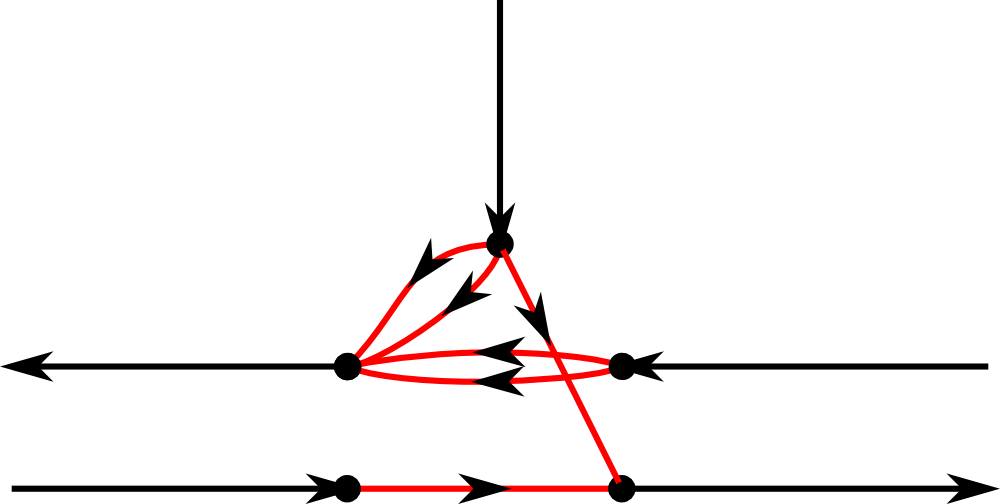
\includegraphics[width=0.4\textwidth]{images/ConnectionNetwork.png}
\caption{Connection network of Figure \ref{fig:Introduction:network}}
\label{fig:Model:Connection}
\end{figure}
\subsection{Traffic Light Phases}
We have a traffic light phase for each connection in a traffic light, and each phase details the light setting for just this one connection.
SUMO limits the allowed light settings to $red$, $yellow$ and $green$.
A phase of a traffic light, $\phase$ is defined as $\langle(\light_0, \ti_0),(\light_1, \ti_1),\dots, (\light_n, \ti_n) \rangle$ where the light setting is $\light_i\in \{red, yellow, green\}$ in $\ti_i$ seconds for $0 \leq i \leq n$.
A connection in an unregulated junction will simply have the phase $\langle(green, \infty)\rangle$
The phases of a traffic light defines the light settings when possible sensors are not triggered. %TODO hm sensors what is that ?


\subsection{Map}
A map is a directed graph, $G = (V, E, C)$ where $V$ is a set of vertices, $E$ is a set of edges representing road segments and $C$ is a set of connections.
Every edge $\edge\in E$ has a starting point \estart, an end point \eend and a maximum speed \espeed. 
The lenght of an edge is the euclidean distance between $\estart$ and \eend denoted as \elength.
In figure~\ref{fig:Introduction:network} we have five egdes, as the road coming from north is unidirectional and six connections assuming one cannot make U-turn.

\subsection{Sensors}
A sensor can detect whether a vehicle is located at the sensor or not. Sensors can be induction loops, video cameras or others.


\subsection{Junction}
We define a junction \ju to be a set of connection $\jucons \subseteq C$. A junction can be either regulated or unregulated. In an unregulated traffic light normal traffic rules apply. In a regulated traffic light vehicles will have to check the phases $\cphase$ of the connection \vehpos. A junction is said to be unregulated iff $\forall c \in \jucons | \cphase = \langle(green, \infty)\rangle$


\begin{comment}
\subsection{Traffic Light}
A traffic light, $\tl$ controls the flow of traffic at a junction, and is associated with a set of connections, $\tlcons$. % and a set of sensors, $\tlsen$.

%TODO: Is this out of place?
A junction has a physical size and geometry, as illustrated in Figure~\ref{fig:Introduction:network}.
In SUMO this is represented as a center point and a geometric object.
To get the distance from a traffic light to a vehicle, we simply calculate the distance to the center of the traffic and substract the average distance from the center to the outer egdes of the traffic light. 
Hence, we cannot predict the precise distance to the position at a traffic light where the driver must stop.
However, there is already inaccuracies due to blocking cars.
This can for example be observed in Figure \ref{fig:Introduction:network} where vehicle $\veh_1$ drives towards traffic light $\tl_2$. %TODO: fix reference
He believes that the distance to were he has to stop is the distance $\dist_1$, however, the two blue cars already waiting in line blocks a part of the road.
\end{comment}

\begin{comment}
\subsection{Trajectory}
A trajectory is the GPS records of the time and location of a vehicle 
\end{comment}

\subsection{Routes}
A route, $\route$, is a sequence of edges on the map, $\langle \edge_1, \edge_2, \dots \edge_n \rangle$, where $\exists \con$ s.t. $\eendi{i} = \cestart$ and $\estarti{i+1} = \ceend$ for $0\leq i< n$.
The vehicle starts at $\edge_1$ and moves along the sequence until $\edge_n$ has been reached.